\documentclass{article}
\usepackage{amssymb}
\usepackage{amsmath}
\usepackage{graphicx}
\usepackage{subcaption}
\title{\textbf{ECE 6560 Final Project - Image Smoothing}}
\author{Alexander Domagala}
\date{Spring 2024}

\begin{document}
  \maketitle

  %%%%%%%%%%%%%%%%%%%%%%%%%%%%%%%%%%%%%%%%%%%%%%%%%%%%%%%%%%%%%%%
  % Problem Description
  %%%%%%%%%%%%%%%%%%%%%%%%%%%%%%%%%%%%%%%%%%%%%%%%%%%%%%%%%%%%%%%
  \section{Problem Description}
  Although image processing techniques began to appear around the 1960s, the proliferation of inexpensive
  digital computing power has greatly widened the application pool. Image processing techniques
  can now be found in areas such as digital photography, medical imaging, and object detection/tracking.\\

  \noindent
  All these applications can be affected by a very common problem: image noise.
  Noise can render further processing ineffective, thus there exist a variety of approaches by which
  we can attempt to smooth and denoise images. More traditional denoising techniques
  may involve fixed convolutional kernels, eg. box blur \cite{Convolution}, that indicate how a specific pixel
  can be updated as a weighted sum of its neighbors. Approaches of this nature will reduce the noise in
  exchange for the image appearing blurred.\\

  \noindent
  We can instead leverage PDEs to describe how an image should be updated depending on its local characteristics.
  Approaches that leverage PDEs offer noise reduction while also lessening the blurring that is done to edges.\\

  \noindent
  In this project, we will explore how we can tailor a PDE-based filter to suit a specific image.
  The goal is that by understanding the characteristics of the image's edges and noise, we
  will be able to outperform a more generalized PDE-based filter. Our filter will be developed
  using techniques falling under Anisotropic Diffusion.



  %%%%%%%%%%%%%%%%%%%%%%%%%%%%%%%%%%%%%%%%%%%%%%%%%%%%%%%%%%%%%%%
  % Mathematical Modeling
  %%%%%%%%%%%%%%%%%%%%%%%%%%%%%%%%%%%%%%%%%%%%%%%%%%%%%%%%%%%%%%%
  \newpage
  \section{Mathematical Modeling}

  %%%%%%%%%%%%%%%%%%%%%%%%%%%%%%
  % Introduction
  %%%%%%%%%%%%%%%%%%%%%%%%%%%%%%
  \subsection{Introduction}
  Before explicitly developing our PDE, we must first understand the behavior that we want our system to have.
  We will leverage the Calculus of Variations. This is a powerful framework that will help arrive at a PDE
  that reflects some desired behavior. Examine the following equation
  \begin{center}
    \begin{tabular}{l}
      $E(I) = \int_{0}^{1} \int_{0}^{1} L(I, I_{x}, I_{y}, x, y) dx dy$
    \end{tabular}
  \end{center}

  \noindent
  $E(I)$ is the energy functional. Similar to the common understanding of a function, it can output
  a single value. The key difference is that the input to the energy functional, is another entire
  function that will depend on traditional variables like $x,y$, etc.\\

  \noindent
  Note that all notation before section (4) is for continuous space: $x,y \in \mathbb{R}$. Thus,
  the input to the energy functional can be thought of as an image with an infinite amount of pixels: $I(x,y)$.\\

  \noindent
  During lecture, the following example was introduced. If we want to measure how noisy a certain image is,
  we could measure the average value of the image's gradient squared.
  \begin{center}
    \begin{tabular}{l}
      $E(I) = \int_{0}^{1} \int_{0}^{1} \frac{1}{2} (\| \nabla_{I} \|)^{2} dx$
    \end{tabular}
  \end{center}

  \noindent
  Given two copies of the same image with different amounts of noise, the noiser image will have larger values
  for $E(I)$ while smoother image will have a smaller values for $E(I)$. The Calculus of Variations says
  that we can utilize the Euler Lagrange equation
  $L_{I} - \frac{\partial}{\partial x}L_{I_{x}} - \frac{\partial}{\partial y}L_{I_{y}} = 0$ to solve an
  optimization problem that minimizes the energy functional $E(I)$. Since we defined the
  energy functional to measure the average gradient squared, minimization will yield a method
  by which we can most efficiently reduce this criterion.\\

  \newpage
  \noindent
  In the case of the example, minimization yields the Linear Heat equation
  \begin{center}
    $I_{t} = \Delta I$
  \end{center}
  The Linear Heat equation optimally reduces the average squared value of the gradient in an image.
  This means that areas of high gradient in the image will be aggresively smoothed. Hence, the edges (which
  are areas of higher gradient) are not very well preserved with this technique.
  \begin{center}
    Quadratic Penalty: $x^2$\\
    \vspace{12pt}
    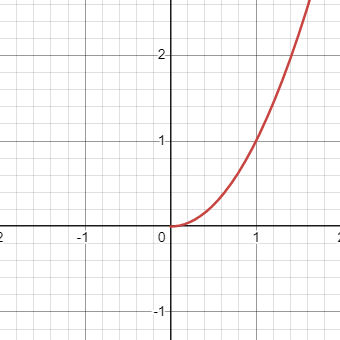
\includegraphics[scale=0.5]{../report_images/squared.png}
  \end{center}
  \vspace{12pt}

  \noindent
  A major improvement is to instead use a linear penalty. Smoothing that takes place at the edges
  will be less extreme than the previous case. This means that enough diffusion could take place
  in areas of low gradient such that the image appears to be denoised. Then, the diffusion can be stopped.
  Although the edges also experience diffusion, the penalty is much more lenient than the previous case.
  This method is known as Total Variation Diffusion.
  \begin{center}
    Linear Penalty: $x$\\
    \vspace{12pt}
    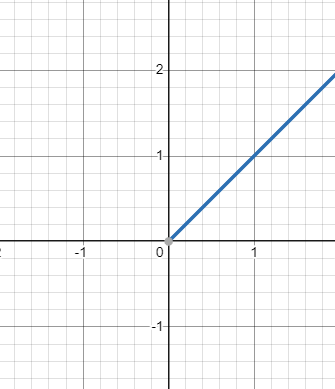
\includegraphics[scale=0.5]{../report_images/linear.png}
  \end{center}

  %%%%%%%%%%%%%%%%%%%%%%%%%%%%%%
  % Anisotropic Diffusion
  %%%%%%%%%%%%%%%%%%%%%%%%%%%%%%
  \newpage
  \noindent
  \subsection{Anisotropic Diffusion}
  The previous examples showed that by selecting a certain penalty and then minimizing the
  associated energy functional, we can control the smoothing behavior of a particular system.
  The examples can be generalized to what is known as Anisotropic or Perona-Malik Diffusion.
  We can continue towards the project goal of tailoring a penalty to a specific image
  by working under this framework.
  \begin{center}
    $E(I) = \iint C(\| \nabla_{I} \|) dx dy$
  \end{center}
  Note that the penalty $C(\| \nabla_{I} \|)$
  must be strictly increasing for the diffusion to be well-posed. We can then
  arrive at our PDE via gradient descent\\

  \begin{center}
    \begin{tabular}{l}
      \vspace{12pt}
      $L(I,I_{x},I_{y},x,y) = C(\| \nabla_{I} \|)$\\
      \vspace{12pt}
      $L_{I} = 0$\\
      \vspace{12pt}
      $L_{I_{x}} = \dot{C}(\| \nabla_{I} \|) \frac{I_{x}}{\| \nabla_{I} \|}$\\
      \vspace{12pt}
      $L_{I_{y}} = \dot{C}(\| \nabla_{I} \|) \frac{I_{y}}{\| \nabla_{I} \|}$\\
      \vspace{12pt}
      $\nabla_{I}E = L_{I} - \frac{\partial}{\partial x}L_{I_{x}} - \frac{\partial}{\partial y}L_{I_{y}}$\\
      \vspace{12pt}
      $I_{t} = -\nabla_{I}E$\\
      \vspace{12pt}
      $I_{t} = -L_{I} + \frac{\partial}{\partial x}L_{I_{x}} + \frac{\partial}{\partial y}L_{I_{y}}$\\
      \vspace{12pt}
      $I_{t} = \frac{\partial}{\partial x}(\dot{C}(\| \nabla_{I} \|) \frac{I_{x}}{\| \nabla_{I} \|}) + \frac{\partial}{\partial y}(\dot{C}(\| \nabla_{I} \|) \frac{I_{y}}{\| \nabla_{I} \|})$\\
      \vspace{12pt}
      $I_{t} = \nabla \cdot (\frac {\dot{C}(\| \nabla_{I} \|)}{\| \nabla_{I} \|} \nabla I)$
    \end{tabular}
  \end{center}

  \noindent
  Now we will work to develop a custom penalty $C(\| \nabla_{I}\|)$ that supports
  enhanced edge preservation for specific images.

  %%%%%%%%%%%%%%%%%%%%%%%%%%%%%%
  % Image Profiling
  %%%%%%%%%%%%%%%%%%%%%%%%%%%%%%
  \newpage
  \subsection{Image Profiling}
  Consider the following images
  \begin{figure}[!htb]
    \begin{center}
      \begin{subfigure}[b]{0.4\textwidth}
        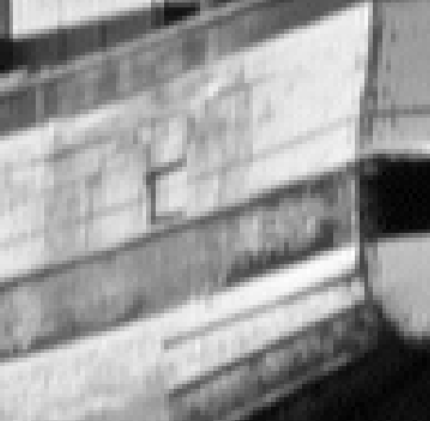
\includegraphics[width=\textwidth]{../report_images/boat_crop.png}
        \caption{Original Image}
      \end{subfigure}
      \hfill
      \begin{subfigure}[b]{0.4\textwidth}
        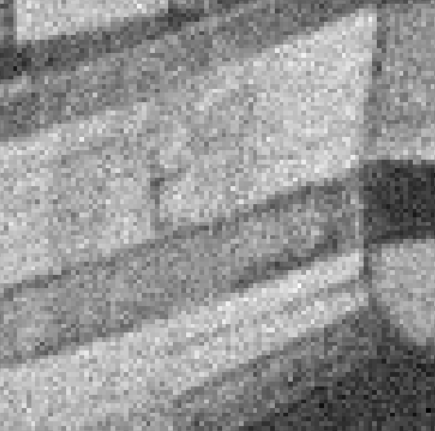
\includegraphics[width=\textwidth]{../report_images/noisy.png}
        \caption{Corrputed Image}
      \end{subfigure}
    \end{center}
  \end{figure}

  \noindent
  We can compute the magnitude gradient at each pixel in the image using the following
  approximations that are derived in section (4):
  \begin{center}
    \begin{tabular}{l}
      \vspace{12pt}
      $I_{x}(x,y,t) = \frac{I(x+\Delta x,y,t) - I(x-\Delta x,y,t)}{2\Delta x}$\\
      \vspace{12pt}
      $I_{y}(x,y,t) = \frac{I(x,y+\Delta y,t) - I(x,y-\Delta y,t)}{2\Delta y}$\\
      $\| \nabla_{I} \| = \sqrt{I_{x}^2 + I_{y}^2}$\\
    \end{tabular}
  \end{center}

  \noindent
  The following image shows the magnitude gradient at each pixel in the noisy image.
  Edges take on a lighter color while darker sections reflect more uniform areas of the image.
  \begin{center}
    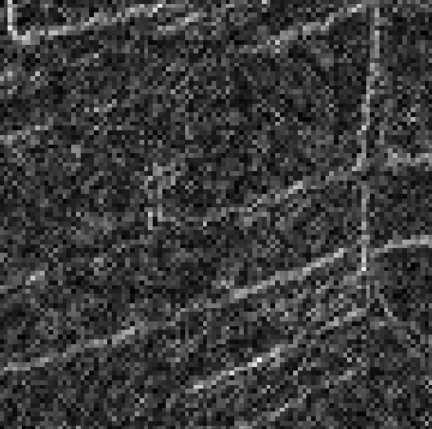
\includegraphics[scale=0.5]{../report_images/noisy_grad.png}
  \end{center}

  \newpage
  \noindent
  The distribution of the magnitude gradient can be visualized using a histogram.
  \begin{center}
    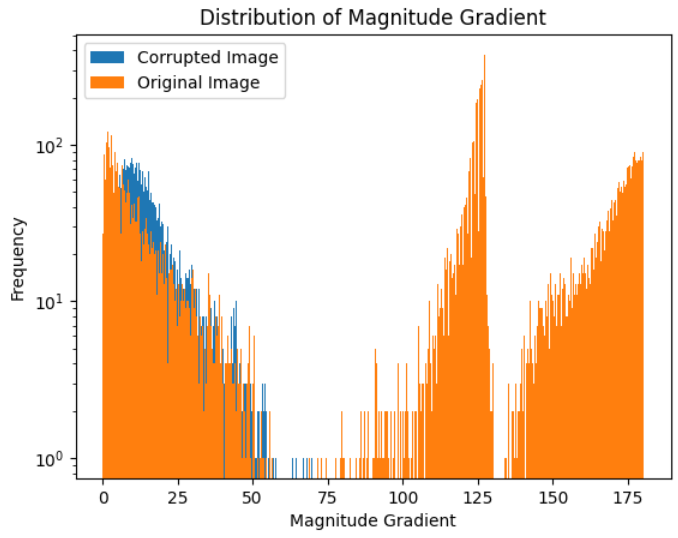
\includegraphics[scale=0.5]{../report_images/gradient.png}
  \end{center}
  \vspace{12pt}

  \noindent
  The corrputed image appears to differ in the range of 80 to 110.
  Let's shape the energy functional so that pixels in the image that
  fall in this range of gradients are smoothed. Thus, we
  can propose the following penalty
  \begin{center}
    Sigmoidal Penalty: $\frac{\lambda}{1+e^{-x}}$\\
    \vspace{12pt}
    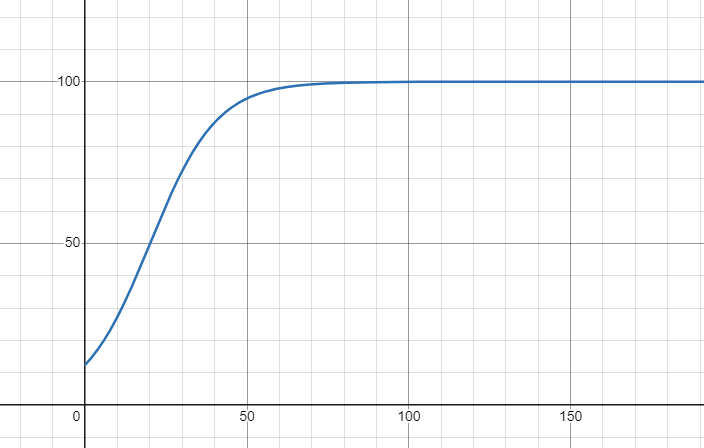
\includegraphics[scale=0.5]{../report_images/sigmoid.png}
  \end{center}
  \vspace{12pt}

  \noindent
  The goal of this penalty is to only have smoothing at the gradients
  that are corrputing the image. By keeping a nearly flat penalty in the for
  the higher gradient, we will greatly reduce the amount of diffusion that
  takes place along the edges.



  %%%%%%%%%%%%%%%%%%%%%%%%%%%%%%%%%%%%%%%%%%%%%%%%%%%%%%%%%%%%%%%
  % Derivation of PDE
  %%%%%%%%%%%%%%%%%%%%%%%%%%%%%%%%%%%%%%%%%%%%%%%%%%%%%%%%%%%%%%%
  \newpage
  \section{Derivation of PDE}

    \noindent Now, recall the Euler-Lagrange equation
      \begin{center}
        \begin{tabular}{l}
          $L_{f} - \frac{\partial}{\partial x}L_{f'} = 0$ (1-D)\\
          $L_{I} - \frac{\partial}{\partial x}L_{I_{x}} - \frac{\partial}{\partial y}L_{I_{y}} = 0$ (2-D)\\
        \end{tabular}
      \end{center}
    \vspace{12pt}

    \noindent
    We can begin working towards obtaining our PDE by setting up a gradient descent
      \begin{center}
        \begin{tabular}{l}
          $I_{t} = -\nabla_{I}E$\\
          $I_{t} = -L_{I} + \frac{\partial}{\partial x}L_{I_{x}} + \frac{\partial}{\partial y}L_{I_{y}}$
        \end{tabular}
      \end{center}
    \vspace{12pt}

    \noindent
    We will now have to compute terms $L_{I}$, $L_{I_{x}}$, $L_{I_{y}}$ using the previously obtained energy functional
      \begin{center}
        \begin{tabular}{l}
          $L(I,I_{x},I_{y},x,y) = \frac{\lambda}{1+e^{\alpha}}$, where $\alpha = -\frac{1}{\beta}(\| \nabla_{I} \|)$\\
          We will also include a term $\epsilon$ such that $\| \nabla_{I} \| = \sqrt{I_{x}^2 + I_{y}^2 + \epsilon^2}$\\
          $\epsilon$ is a constant used to prevent stability issues and will be examined more\\
          \vspace{12pt}
          closely in section (4).\\
          $L_{I} = \frac{\partial}{\partial I}(L)$\\
          $L_{I} = 0$\\
          $L_{I_{x}} = \frac{\partial}{\partial I_{x}}(L)$\\
          $L_{I_{x}} = \frac{\lambda}{\beta} \frac{e^\alpha}{(1+e^{\alpha})^2} \frac{I_{x}}{\sqrt{I_{x}^2 + I_{y}^2 + \epsilon^2}}$\\
          $L_{I_{y}} = \frac{\partial}{\partial I_{y}}(L)$\\
          $L_{I_{y}} = \frac{\lambda}{\beta} \frac{e^\alpha}{(1+e^{\alpha})^2} \frac{I_{y}}{\sqrt{I_{x}^2 + I_{y}^2 + \epsilon^2}}$\\
        \end{tabular}
      \end{center}
      \vspace{12pt}

    \noindent
    Now that we have obtained our expressions for $L_{I_{x}}$ and $L_{I_{y}}$, we must compute their partial derivatives
    as shown by the Euler-Lagrange equation. This will be shown for $\frac{\partial}{\partial x}L_{I_{x}}$. $\frac{\partial}{\partial y}L_{I_{y}}$ will be obtained by examining
    the expression of $\frac{\partial}{\partial x}L_{I_{x}}$.\\

    \noindent
    Let $\phi$ denote $\frac{e^\alpha}{(1+e^{\alpha})^2}$ and let $\gamma$ denote $\frac{I_{x}}{\sqrt{I_{x}^2 + I_{y}^2 + \epsilon^2}}$.
    We can begin finding $\frac{\partial}{\partial x}L_{I_{x}}$ by using the product-rule $\frac{\partial}{\partial x}(\gamma)\phi + \frac{\partial}{\partial x}(\phi)\gamma$.
    We will start with the left side of the sum. Note that we must include $\frac{\lambda}{\beta}$ in the final expression.\\
    \begin{center}
      \begin{tabular}{l}
        \vspace{12pt}
        $\frac{\partial}{\partial x}(\gamma)\phi$\\
        \vspace{12pt}
        $\frac{\partial}{\partial x}(\frac{I_{x}}{\sqrt{I_{x}^2 + I_{y}^2 + \epsilon^2}})\phi$\\
        $(\frac{I_{xx}}{(I_{x}^2 + I_{y}^2 + \epsilon^2)^\frac{1}{2}} + \frac{I_{x}}{(I_{x}^2 + I_{y}^2 + \epsilon^2)^\frac{3}{2}}(I_{x}I_{xx} + I_{y}I_{xy}))\phi$
      \end{tabular}
    \end{center}
    \vspace{12pt}
    
    \newpage
    \noindent
    We can now examine the right side of $\frac{\partial}{\partial x}(\gamma)\phi + \frac{\partial}{\partial x}(\phi)\gamma$.
    \begin{center}
      \begin{tabular}{l}
        $\frac{\partial}{\partial x}(\phi)\gamma$\\
        $\frac{\partial}{\partial x}(\frac{e^\alpha}{(1+e^{\alpha})^2})\gamma$\\
        $\frac{\partial}{\partial x}((e^\alpha)(1+e^{\alpha})^{-2})\gamma$\\
      \end{tabular}
    \end{center}

    \noindent
    We see that we will need to again perform the product-rule between $(e^\alpha)$ and\\
    $(1+e^{\alpha})^{-2}$. Taking the partial derivative of $(e^\alpha)$
    \begin{center}
      \begin{tabular}{l}
        $-\frac{1}{\beta} e^{\alpha} \frac{1}{(I_{x}^2 + I_{y}^2 + \epsilon^2)^\frac{1}{2}} (I_{x}I_{xx}+I_{y}I_{xy})$
      \end{tabular}
    \end{center}

    \noindent
    Taking the partial derivative of $(1+e^{\alpha})^{-2}$
    \begin{center}
      \begin{tabular}{l}
        $-2(1+e^{\alpha})^{-3} (-\frac{1}{\beta} e^{\alpha} \frac{1}{(I_{x}^2 + I_{y}^2 + \epsilon^2)^\frac{1}{2}} (I_{x}I_{xx}+I_{y}I_{xy})) $
      \end{tabular}
    \end{center}

    \noindent
    Thus, after factoring common terms, $\frac{\partial}{\partial x}((e^\alpha)(1+e^{\alpha})^{-2})$ yields
    \begin{center}
      \begin{tabular}{l}
        $[-\frac{1}{\beta} (e^\alpha) (\frac{1}{(I_{x}^2 + I_{y}^2 + \epsilon^2)^\frac{1}{2}}) (I_{x}I_{xx}+I_{y}I_{xy})] [(1+e^{\alpha})^{-2} + (e^\alpha)(-2(1+e^{\alpha})^{-3})]$\\
      \end{tabular}
    \end{center}
    \vspace{12pt}
    \vspace{12pt}

  \noindent
  We have reached the final expression for $\frac{\partial}{\partial x}L_{I_{x}}$
  \begin{center}
    \begin{tabular}{l}
      \vspace{12pt}
      $\frac{\partial}{\partial x}L_{I_{x}} =$\\
      \vspace{12pt}
      $\frac{\lambda}{\beta}[ (\frac{I_{xx}}{(I_{x}^2 + I_{y}^2 + \epsilon^2)^\frac{1}{2}}) - (\frac{I_{x}}{(I_{x}^2 + I_{y}^2 + \epsilon^2)^\frac{3}{2}}) (I_{x}I_{xx} + I_{y}I_{xy}) (\frac{e^\alpha}{(1+e^{\alpha})^2}) +$\\
      \vspace{12pt}
      $(\frac{I_{x}}{(I_{x}^2 + I_{y}^2 + \epsilon^2)^\frac{1}{2}}) [-\frac{1}{\beta} (e^\alpha) (\frac{1}{(I_{x}^2 + I_{y}^2 + \epsilon^2)^\frac{1}{2}}) (I_{x}I_{xx}+I_{y}I_{xy})] [(1+e^{\alpha})^{-2} + (e^\alpha)(-2(1+e^{\alpha})^{-3})]]$
    \end{tabular}
  \end{center}
  \vspace{12pt}

  \noindent
    $\frac{\partial}{\partial y}L_{I_{y}}$ can be obtained by modifying $\frac{\partial}{\partial x}L_{I_{x}}$
    \begin{center}
      \begin{tabular}{l}
        \vspace{12pt}
        $\frac{\partial}{\partial y}L_{I_{y}} =$\\
        \vspace{12pt}
        $\frac{\lambda}{\beta}[ (\frac{I_{yy}}{(I_{x}^2 + I_{y}^2 + \epsilon^2)^\frac{1}{2}}) - (\frac{I_{y}}{(I_{x}^2 + I_{y}^2 + \epsilon^2)^\frac{3}{2}}) (I_{x}I_{xy} + I_{y}I_{yy}) (\frac{e^\alpha}{(1+e^{\alpha})^2}) +$\\
        \vspace{12pt}
        $(\frac{I_{y}}{(I_{x}^2 + I_{y}^2 + \epsilon^2)^\frac{1}{2}}) [-\frac{1}{\beta} (e^\alpha) (\frac{1}{(I_{x}^2 + I_{y}^2 + \epsilon^2)^\frac{1}{2}}) (I_{x}I_{xy}+I_{y}I_{yy})] [(1+e^{\alpha})^{-2} + (e^\alpha)(-2(1+e^{\alpha})^{-3})]]$
      \end{tabular}
    \end{center}
    \vspace{12pt}

    \newpage
    \noindent
    Our final gradient-descent PDE is
    \begin{center}
      \begin{tabular}{l}
        \vspace{12pt}
        $I_{t} = \frac{\lambda}{\beta}[ (\frac{I_{xx}}{(I_{x}^2 + I_{y}^2 + \epsilon^2)^\frac{1}{2}}) - (\frac{I_{x}}{(I_{x}^2 + I_{y}^2 + \epsilon^2)^\frac{3}{2}}) (I_{x}I_{xx} + I_{y}I_{xy}) (\frac{e^\alpha}{(1+e^{\alpha})^2}) +$\\
        \vspace{12pt}
        $(\frac{I_{x}}{(I_{x}^2 + I_{y}^2 + \epsilon^2)^\frac{1}{2}}) [-\frac{1}{\beta} (e^\alpha) (\frac{1}{(I_{x}^2 + I_{y}^2 + \epsilon^2)^\frac{1}{2}}) (I_{x}I_{xx}+I_{y}I_{xy})] [(1+e^{\alpha})^{-2} + (e^\alpha)(-2(1+e^{\alpha})^{-3})]+ $\\
        \vspace{12pt}
        $(\frac{I_{yy}}{(I_{x}^2 + I_{y}^2 + \epsilon^2)^\frac{1}{2}}) - (\frac{I_{y}}{(I_{x}^2 + I_{y}^2 + \epsilon^2)^\frac{3}{2}}) (I_{x}I_{xy} + I_{y}I_{yy}) (\frac{e^\alpha}{(1+e^{\alpha})^2}) +$\\
        \vspace{12pt}
        $(\frac{I_{y}}{(I_{x}^2 + I_{y}^2 + \epsilon^2)^\frac{1}{2}}) [-\frac{1}{\beta} (e^\alpha) (\frac{1}{(I_{x}^2 + I_{y}^2 + \epsilon^2)^\frac{1}{2}}) (I_{x}I_{xy}+I_{y}I_{yy})] [(1+e^{\alpha})^{-2} + (e^\alpha)(-2(1+e^{\alpha})^{-3})]]$
        \vspace{12pt}
      \end{tabular}
    \end{center}

    \noindent
    Where $\alpha = -\frac{1}{\beta}(\| \nabla_{I} \|)$ and $\| \nabla_{I} \| = \sqrt{I_{x}^2 + I_{y}^2 + \epsilon^2}$\\



  %%%%%%%%%%%%%%%%%%%%%%%%%%%%%%%%%%%%%%%%%%%%%%%%%%%%%%%%%%%%%%%
  % Discretization and Implementation
  %%%%%%%%%%%%%%%%%%%%%%%%%%%%%%%%%%%%%%%%%%%%%%%%%%%%%%%%%%%%%%%
  \newpage
  \section{Discretization and Implementation}
  \noindent
  The PDE that was obtained in the previous section is only applicable for continuous
  time and space variables. We must discretize the PDE so that it can actually be implemented in software.\\

  %%%%%%%%%%%%%%%%%%%%%%%%%%%%%%
  % Numerical Differentiation
  %%%%%%%%%%%%%%%%%%%%%%%%%%%%%%
  \subsection{Numerical Differentiation}
  \noindent
  Before explicitly discretizing the PDE, we must also obtain numeric approximations for its partial
  derivatives. Beginning with the left side of the PDE, let's approximate $I_{t}$. 
  It is important to understand that the PDE is defining how the image will be smoothed
  over successive iterations. In other words, it specifies how the image is updated as time increases.
  Thus, it is appropriate to use a forward difference.\\

  \noindent
  The forward difference for a single (space) variable can be obtained using the 
  numeric differentiation method shown in lecture
  \begin{center}
    \begin{tabular}{l}
      \vspace{12pt}
      $f(x,t) = f(x,t)$\\
      $f(x,t+\Delta t) = f(x,t) + \Delta t f'(x,t) + O(\Delta t^2)$\\
    \end{tabular}
  \end{center}

  \noindent
  After eliminating $f(x,t)$ terms on the right side of the above equations,
  we obtain our approximation. Note that the approximation includes an error term $O(\Delta t)$.
  \begin{center}
    \begin{tabular}{l}
      $f'(x,t) = \frac{f(x,t+\Delta t) - f(x,t)}{\Delta t}$\\
    \end{tabular}
  \end{center}

  \noindent
  Expanding this process to two (space) dimensions yields
  \begin{center}
    \begin{tabular}{l}
      $I_{t}(x,y,t) = \frac{I(x,y,t+\Delta t) - I(x,y,t)}{\Delta t}$\\
    \end{tabular}
  \end{center}
  \vspace{12pt}

  \noindent
  Continuing with the right side of the PDE, approximations are needed for the following partial
  derivatives: $I_{x}$, $I_{y}$, $I_{xx}$, $I_{yy}$, and $I_{xy}$. Since these approximations
  capture how the image is changing with respect to space, it is more appropriate to use a
  central difference rather than a forward difference.\\
  
  \noindent
  Suppose we are trying to approximate
  $I_{x}$. A forward difference would introduce some bias because the value of $I_{x}$ at
  a certain point is dependent on an adjacent image value in the positive x-direction only.
  The central difference will balance out the value of $I_{x}$ since both directions
  are considered. The intent is to make the approximation more robust to variations in image content. \\

  \newpage
  \noindent
  The central difference for a single (space) variable can be obtained using the
  numeric differentiation method shown in lecture
  \begin{center}
    \begin{tabular}{l}
      \vspace{12pt}
      $f(x,t) = f(x,t)$\\
      \vspace{12pt}
      $f(x+\Delta x,t) = f(x,t) + \Delta x f'(x,t) + O(\Delta x^2)$\\
      \vspace{12pt}
      $f(x-\Delta x,t) = f(x,t) - \Delta x f'(x,t) + O(\Delta x^2)$\\
    \end{tabular}
  \end{center}

  \noindent
  After eliminating $f(x,t)$ terms on the right side of the above equations,
  we obtain our approximation. Note that the approximation includes an error term $O(\Delta x)$.
  \begin{center}
    \begin{tabular}{l}
      \vspace{12pt}
      $f'(x,t) = \frac{f(x+\Delta x,t) - f(x-\Delta x,t)}{2\Delta x}$\\
    \end{tabular}
  \end{center}

  \noindent
  Expanding this process to two (space) dimensions yields
  \begin{center}
    \begin{tabular}{l}
      \vspace{12pt}
      $I_{x}(x,y,t) = \frac{I(x+\Delta x,y,t) - I(x-\Delta x,y,t)}{2\Delta x}$\\
      \vspace{12pt}
      $I_{y}(x,y,t) = \frac{I(x,y+\Delta y,t) - I(x,y-\Delta y,t)}{2\Delta y}$\\
    \end{tabular}
  \end{center}

  \noindent
  In order to obtain approximations for $I_{xx}$ and $I_{yy}$, we can simply add additional
  terms to the Taylor Series expansion and then repeat the elimination process
  \begin{center}
    \begin{tabular}{l}
      \vspace{12pt}
      $I_{xx}(x,y,t) = \frac{I(x+\Delta x,y,t) - 2I(x,y,t) + I(x-\Delta x,y,t)}{\Delta x^{2}}$\\
      \vspace{12pt}
      $I_{yy}(x,y,t) = \frac{I(x,y+\Delta y,t) - 2I(x,y,t) + I(x,y-\Delta y,t)}{\Delta y^{2}}$\\
    \end{tabular}
  \end{center}
  \vspace{12pt}

  \noindent
  Finally, we need to obtain an approximation for the mixed partial derivative $I_{xy}$.
  This is achieved by taking the central difference approximation for $I_{x}$ and 
  applying another central difference with respect to $y$
  \begin{center}
    \begin{tabular}{l}
      \vspace{12pt}
      $I_{x}(x,y,t) = \frac{I(x+\Delta x,y,t)}{2\Delta x} - \frac{I(x-\Delta x,y,t)}{2\Delta x}$\\
      \vspace{12pt}
      $I_{xy}(x,y,t) = \frac{\partial}{\partial y}(\frac{I(x+\Delta x,y,t)}{2\Delta x}) - \frac{\partial}{\partial y}(\frac{I(x-\Delta x,y,t)}{2\Delta x})$\\
      \vspace{12pt}
      $I_{xy}(x,y,t) = \frac{1}{2\Delta y}(\frac{I(x+\Delta x,y+\Delta y,t)}{2\Delta x} - \frac{I(x+\Delta x,y-\Delta y,t)}{2\Delta x}) - \frac{1}{2\Delta y}(\frac{I(x-\Delta x,y+\Delta y,t)}{2\Delta x} - \frac{I(x-\Delta x,y-\Delta y,t)}{2\Delta x})$\\
      \vspace{12pt}
      $I_{xy}(x,y,t) = \frac{I(x+\Delta x,y+\Delta y,t) - I(x+\Delta x,y-\Delta y,t) - I(x-\Delta x,y+\Delta y,t) + I(x-\Delta x,y-\Delta y,t)}{4 \Delta x\Delta y} $ \\
    \end{tabular}
  \end{center}

  %%%%%%%%%%%%%%%%%%%%%%%%%%%%%%
  % Parameter Selection
  %%%%%%%%%%%%%%%%%%%%%%%%%%%%%%
  \newpage
  \subsection{Parameter Selection}
  \noindent
  Now that we have obtained all the necessary numeric approximations of the partial derivatives, we
  can move towards defining a scheme that discretizes the PDE. This involves selecting
  some important parameters.\\

  \noindent
  First, we will examine what is an appropriate time-step $\Delta t$. Previously,
  we defined $I_{t}(x,y,t) = \frac{I(x,y,t+\Delta t) - I(x,y,t)}{\Delta t}$. In our implementation,
  $\Delta t$ will multiply the right side of the PDE. The product will then be added to
  the current image to obtain the updated image. Thus, we must find a CFL condition
  so that we can find an appropriate time-step. Recall that during the derivation of
  the PDE, a term $\epsilon$ was included so that $\| \nabla_{I} \| = \sqrt{I_{x}^2 + I_{y}^2 + \epsilon^2}$.
  Suppose the gradient became very small, all terms $I_{x}$ and $I_{y}$ in the PDE would go to zero and 
  we would be left with $I_{t} = \frac{\lambda}{\beta}[(\frac{I_{xx}+I_{yy}}{(\epsilon^2)^\frac{1}{2}})]$.
  Then we simply have the heat equation
  \begin{center}
    \begin{tabular}{l}
      $I_{t} = \frac{\lambda}{\beta \epsilon}\Delta I$
    \end{tabular}
  \end{center}

  \noindent
  We can include our constants with the form of the CFL condition for the two-dimensional linear heat equation
  as shown in lecture
  \begin{center}
    \begin{tabular}{l}
      \vspace{12pt}
      $\frac{\lambda}{\beta \epsilon} \leq \frac{1}{4} \Delta x^2$\\
      $\Delta t \leq \frac{1}{4} \frac{\beta \epsilon}{\lambda} \Delta x^2$\\
    \end{tabular}
  \end{center}

  \noindent
  With a bound set for  $\Delta t$, we can now shift our focus to $\Delta x$ and $\Delta y$. Since
  a digital image is composed of a finite number of individual pixels, we will compute the different
  partial derivative approximations by simply taking our current pixel and applying an offset of
  +1 or -1 to the current pixel's $x$ and $y$ indices. For example, for $I_{x}$
  \begin{center}
    \begin{tabular}{l}
      $I_{x}(x,y,t) = \frac{I(x+\Delta x,y,t)}{2\Delta x} - \frac{I(x-\Delta x,y,t)}{2\Delta x}$, we can
      \vspace{12pt}
      compute $I_{x}$ at pixel $(a,b)$ as\\
      $I_{x}(a,b,t) = \frac{I(a+1,b,t)}{2(1)} - \frac{I(a-1,b,t)}{2(1)}$
    \end{tabular}
  \end{center}

  \noindent
  Finally, we will iterate through each pixel in the image and compute how the pixel should
  be updated based on the PDE.

  %%%%%%%%%%%%%%%%%%%%%%%%%%%%%%
  % Implementation Summary
  %%%%%%%%%%%%%%%%%%%%%%%%%%%%%%
  \newpage
  \subsection{Implementation Summary}
  \noindent
  \vspace{12pt}
  \textbf{PDE}\\
  \begin{tabular}{l}
    \vspace{12pt}
    $I_{t} = \frac{\lambda}{\beta}[ (\frac{I_{xx}}{(I_{x}^2 + I_{y}^2 + \epsilon^2)^\frac{1}{2}}) - (\frac{I_{x}}{(I_{x}^2 + I_{y}^2 + \epsilon^2)^\frac{3}{2}}) (I_{x}I_{xx} + I_{y}I_{xy}) (\frac{e^\alpha}{(1+e^{\alpha})^2}) +$\\
    \vspace{12pt}
    $(\frac{I_{x}}{(I_{x}^2 + I_{y}^2 + \epsilon^2)^\frac{1}{2}}) [-\frac{1}{\beta} (e^\alpha) (\frac{1}{(I_{x}^2 + I_{y}^2 + \epsilon^2)^\frac{1}{2}}) (I_{x}I_{xx}+I_{y}I_{xy})] [(1+e^{\alpha})^{-2} + (e^\alpha)(-2(1+e^{\alpha})^{-3})]+ $\\
    \vspace{12pt}
    $(\frac{I_{yy}}{(I_{x}^2 + I_{y}^2 + \epsilon^2)^\frac{1}{2}}) - (\frac{I_{y}}{(I_{x}^2 + I_{y}^2 + \epsilon^2)^\frac{3}{2}}) (I_{x}I_{xy} + I_{y}I_{yy}) (\frac{e^\alpha}{(1+e^{\alpha})^2}) +$\\
    \vspace{12pt}
    $(\frac{I_{y}}{(I_{x}^2 + I_{y}^2 + \epsilon^2)^\frac{1}{2}}) [-\frac{1}{\beta} (e^\alpha) (\frac{1}{(I_{x}^2 + I_{y}^2 + \epsilon^2)^\frac{1}{2}}) (I_{x}I_{xy}+I_{y}I_{yy})] [(1+e^{\alpha})^{-2} + (e^\alpha)(-2(1+e^{\alpha})^{-3})]]$\\
    \vspace{12pt}
    Where $\alpha = -\frac{1}{\beta}(\| \nabla_{I} \|)$ and $\| \nabla_{I} \| = \sqrt{I_{x}^2 + I_{y}^2 + \epsilon^2}$\\
  \end{tabular}
  \vspace{12pt}

  \noindent
  \vspace{12pt}
  \textbf{Partial Derivatives}\\
  \begin{tabular}{l}
    \vspace{12pt}
    $I_{t}(x,y,t) = \frac{I(x,y,t+\Delta t) - I(x,y,t)}{\Delta t}$\\
    \vspace{12pt}
    $I_{x}(x,y,t) = \frac{I(x+\Delta x,y,t)}{2\Delta x} - \frac{I(x-\Delta x,y,t)}{2\Delta x}$\\
    \vspace{12pt}
    $I_{y}(x,y,t) = \frac{I(x,y+\Delta y,t) - I(x,y-\Delta y,t)}{2\Delta y}$\\
    \vspace{12pt}
    $I_{xx}(x,y,t) = \frac{I(x+\Delta x,y,t) - 2I(x,y,t) + I(x-\Delta x,y,t)}{\Delta x^{2}}$\\
    \vspace{12pt}
    $I_{yy}(x,y,t) = \frac{I(x,y+\Delta y,t) - 2I(x,y,t) + I(x,y-\Delta y,t)}{\Delta y^{2}}$\\
    \vspace{12pt}
    $I_{xy}(x,y,t) = \frac{I(x+\Delta x,y+\Delta y,t) - I(x+\Delta x,y-\Delta y,t) - I(x-\Delta x,y+\Delta y,t) + I(x-\Delta x,y-\Delta y,t)}{4 \Delta x\Delta y} $ \\
  \end{tabular}
  \vspace{12pt}

  \newpage
  \noindent
  \vspace{12pt}
  \textbf{CFL Condition}\\
  \begin{tabular}{l}
    \vspace{12pt}
    $\Delta t \leq \frac{1}{4} \frac{\beta \epsilon}{\lambda} \Delta x^2$\\
  \end{tabular}
  \vspace{12pt}

  \noindent
  \vspace{12pt}
  \textbf{Parameters}\\
  \begin{tabular}{l}
    \vspace{12pt}
    $\Delta t, \Delta x, \Delta y, \beta, \epsilon, \lambda $\\
  \end{tabular}
  \vspace{12pt}

  \noindent
  \vspace{12pt}
  \textbf{Format of Implemented PDE}\\
  \begin{tabular}{l}
    \vspace{12pt}
    $I(x,y,t+\Delta t) = I(x,y,t) + \Delta t (I_{t})$\\
  \end{tabular}
  \vspace{12pt}



  %%%%%%%%%%%%%%%%%%%%%%%%%%%%%%%%%%%%%%%%%%%%%%%%%%%%%%%%%%%%%%%
  % Experiment
  %%%%%%%%%%%%%%%%%%%%%%%%%%%%%%%%%%%%%%%%%%%%%%%%%%%%%%%%%%%%%%%
  \newpage
  \section{Experiment}
  
  %%%%%%%%%%%%%%%%%%%%%%%%%%%%%%
  % Procedure
  %%%%%%%%%%%%%%%%%%%%%%%%%%%%%%
  \subsection{Procedure}
  \begin{enumerate}
    \item Select image and load into program.
    \item Run gradient histogram to understand characteristics of image.
    \item Update smoothing parameters.
    \item Run smoothing algorithm on image, measure and record MSE during each iteration.
    \item After MSE reaches minimum and begins to increase, run 20 iterations past this point.
  \end{enumerate}

  %%%%%%%%%%%%%%%%%%%%%%%%%%%%%%
  % Results
  %%%%%%%%%%%%%%%%%%%%%%%%%%%%%%
  \newpage
  \subsection{Results}


  %%%%%%%%%%%%%%%%%%%%%%%%%%%%%%%%%%%%%%%%%%%%%%%%%%%%%%%%%%%%%%%
  % Conclusion
  %%%%%%%%%%%%%%%%%%%%%%%%%%%%%%%%%%%%%%%%%%%%%%%%%%%%%%%%%%%%%%%
  \section{Conclusion}


  \begin{thebibliography}{unsrt}
    \bibitem{Thomas_book}
      Thomas, L. \& Ari, R. d. \emph{Biological Feedback} (CRC Press, USA, 1990).
    \bibitem{Convolution}
      %https://web.archive.org/web/20060718054020/http://www.acm.uiuc.edu/siggraph/workshops/wjarosz_convolution_2001.pdf
      Thomas, L. \& Ari, R. d. \emph{Biological Feedback} (CRC Press, USA, 1990).
  \end{thebibliography}

\end{document}